\section{Rows of engines: the stacked-chip relay}\label{sec:rows}

One focal-plane engine steers one row of tweezers along $x$. This section describes how 16 such chips are
stacked and imaged onto the atoms as 16 independent rows, what the collimator in front of each chip must do,
and how the rows are kept mutually incoherent without one frequency shifter per chip.

The result is as follows. Sixteen chips of design D1 (128 input ports, 192 arms and emitters,
Sec.~\ref{sec:engine}), stacked at 0.5~mm pitch, each with its own fast-axis collimator (FAC), are imaged as
16 rows 4~\textmu m apart through the NA~0.5 objective at 1064.4~nm. The adopted collimator is a glued
Weierstrass block followed by a two-asphere aplanat. With it, a 1.2~mK tweezer needs 57~mW of laser power.
A full row produces a crosstalk of $1.8\times10^{-4}$ at the neighbouring row (ideal collimator). Rows are as independent as
the tweezers within a row provided their relative optical phase is randomised much faster than the trap
period. One phase modulator on the common seed, driven with Gaussian noise, together with different fibre
delays per chip, does this. The costs are a collimator alignment of $\pm0.1$~\textmu m in height, a
diffraction-limited collimator at NA~0.9, and two rules on spectral filtering and parasitic reflections in
the laser chain. All values are simulated in scalar wave optics (with ray tracing and 2D FDTD where stated)
or derived from those simulations; the code and results are listed in \texttt{docs/stacked\_relay.md},
\texttt{docs/collimator.md}, \texttt{docs/row\_coherence.md} and \texttt{docs/pm\_am.md}.

\subsection{Anamorphic layout}\label{sec:rows-layout}

The relay treats the two axes differently. In $x$, the relay of Sec.~\ref{sec:engine} images the emitter plane
onto the objective pupil, so the atoms see the far field of the chip. In $y$, each chip's facet sits in the
front focal plane of its own cylindrical collimator. The back focal planes of the collimators form a plane
$S$, which a common $y$ lens group of effective focal length $F_y$ Fourier transforms onto the pupil. Thus $S$
is imaged onto the atoms with magnification $f_\mathrm{obj}/F_y = 1/D$, and chip $m$ lands at
$y_m = m\,d_c/D$. Here, $d_c$ is the chip pitch, $D$ the demagnification of the stack, and
$f_\mathrm{obj}=17.3$~mm the objective focal length (pupil radius $f_\mathrm{obj}\,\mathrm{NA}$ at a working
distance of 15~mm). At the same time, the pupil is an image of the facet in both axes, with magnification 60
in $x$ and 12,400 in $y$. Because each chip has its own collimator centred on its facet, all 16 facet images
overlap in the pupil, and the row offsets come only from the tilt $y_m/F_y$. A single common collimator would
not work: it would place the 16 facet images side by side in the pupil.

The free parameter of the $y$ design is the pupil radius referred back to the facet,
$\beta = \mathrm{NA}\,f_\mathrm{FAC}/D$. Here, $f_\mathrm{FAC}$ is the collimator focal length and NA~$=0.5$.
The parameter $\beta$ plays the role of the pupil fill (Sec.~\ref{sec:rows-fill}). The row pitch fixes $D$,
and $\beta$ then fixes $f_\mathrm{FAC}$. Table~\ref{tab:rows-layout} gives the first-order layout for
$\beta = 0.7$~\textmu m (thin cylindrical lenses; ABCD matrices of both axes checked).

\begin{table}[htbp]\centering\small
\caption{First-order layout of the anamorphic relay for 16 chips at 0.5~mm pitch, $\beta=0.7$~\textmu m,
FAC NA~0.9. Thin lenses; derived. The 4~\textmu m row pitch is the design point.}
\label{tab:rows-layout}
\begin{tabular}{cccccc}
\toprule
row pitch & $D$ & $F_y$ & $f_\mathrm{FAC}$ & collimated half-height & facet to pupil \\
\midrule
3~\textmu m & 167 & 2.89~m & 233~\textmu m & 210~\textmu m & 439~mm \\
4~\textmu m & 125 & 2.17~m & 175~\textmu m & 158~\textmu m & 382~mm \\
5~\textmu m & 100 & 1.73~m & 140~\textmu m & 126~\textmu m & 347~mm \\
6~\textmu m & 83 & 1.44~m & 117~\textmu m & 105~\textmu m & 324~mm \\
\bottomrule
\end{tabular}
\end{table}

At 4~\textmu m row pitch ($D=125$), the long effective focal length is realised as a $25\times$ demagnifying
$y$ telescope (focal lengths 100~mm and 4~mm) followed by an 86.6~mm Fourier lens. The $x$ relay is a 4f pair
(3.12~mm and 187.7~mm) with the Fourier slit 6.2~mm from the facets. Both pupils coincide 382~mm from the
facets. The Lagrange invariant matches on both sides: a stack half-height of 4~mm times a collimated NA of
0.0022 equals the atom half-field of 30~\textmu m times 0.5 times the fill. The collimated beams
(158~\textmu m half-height) fit within the 250~\textmu m half-pitch, as they do at 3~\textmu m row pitch
(210~\textmu m). This layout is first order; a real lens design of the anamorphic relay over its 8~mm field
has not been made.

\subsection{Facet mode, pupil fill and crosstalk floor}\label{sec:rows-fill}

\paragraph{Validity of the $y$ results.} All $y$-axis results of this section (pupil fill, collimator
performance, row crosstalk and alignment tolerances) were computed for light with no $x$ direction component,
$s_x=0$. However, a tweezer at position $x_a$ along the row is made of light with $s_x = x_a/288$~\textmu m
(for D1), and the cylindrical collimator then acts with effective indices $\sqrt{n^2-s_x^2}$. The adopted
collimator (Sec.~\ref{sec:rows-collimator}) therefore defocuses the facet by $-99\,s_x^2$~\textmu m. The $y$
figures below hold near the row centre only: the peak falls to 0.97 at $x_a=30$~\textmu m and to 0.48 at
60~\textmu m. With the best common focus offset, a row is usable over $|x_a|\le 45$~\textmu m, less than the
$\pm60$~\textmu m row of D1 used in the crosstalk tests below. Section~\ref{sec:combine} gives the details.

\paragraph{The facet.} The D1 emitter facet ($1.2\times0.4$~\textmu m SiN in oxide) has a vertical mode of
$1/e^2$ equivalent radius 0.39~\textmu m. It radiates into air with a far-field $1/e^2$ half-angle of
$\sin\theta=0.86$. A collimator of NA~0.8 captures 96\% of this light, one of NA~0.9 captures 98.8\%.
Thinning the SiN at the facet expands the vertical mode, but it also expands the lateral one. At 100~nm the
far-field NA drops to 0.51, but the coupling length of adjacent emitters (0.3~\textmu m gap, 1.5~\textmu m
pitch) falls from 228~\textmu m to 47~\textmu m, which leaves no room for an adiabatic vertical taper. The
dense emitter array and a large vertical facet mode are therefore in conflict. We keep the 400~nm facet and
accept the alignment tolerances it sets (Sec.~\ref{sec:rows-align}), which scale as the vertical mode radius
(decentre) and its square (focus).

\paragraph{Pupil fill.} The $y$ profile at the atoms is the facet's far field, clipped by the collimator
aperture and scaled by $\beta/\mathrm{NA}$, then low-pass filtered by the pupil. Crosstalk between rows has
two sources: (i) at small $\beta$, the pupil clips the sharply peaked image of the facet; (ii) at large
$\beta$, the collimator aperture cuts the wide far field with a hard edge, and the pupil makes this edge ring.
As can be seen from Table~\ref{tab:rows-fill} and Fig.~\ref{fig:rows-fill}, the two sources balance near
$\beta=0.7$~\textmu m, which we adopt. Raising the collimator NA to 0.95 lowers the crosstalk at 4~\textmu m
to $7.4\times10^{-5}$. A graded (raised-cosine) collimator edge removes source (ii), but it costs 7 to 8\% of
the light and reaches only $9.4\times10^{-5}$ at 4~\textmu m (at $\beta=0.8$~\textmu m). None of these
options gets below about $5\times10^{-5}$ at 4~\textmu m. This floor is adequate for mutually incoherent rows
(Sec.~\ref{sec:rows-crosstalk}) but not for coherent ones.

\begin{table}[htbp]\centering\small
\caption{Pupil fill scan for an ideal FAC of NA~0.9, single tweezer, 1D ($y$ only), $s_x=0$. Power is
relative to a Gaussian cross axis of $w_0=1.04$~\textmu m (1.22~\textmu m FWHM), the assumption used before
this module. Simulated.}
\label{tab:rows-fill}
\begin{tabular}{cccccc}
\toprule
$\beta$ & cross-axis & $y$ FWHM & power vs & \multicolumn{2}{c}{row crosstalk at} \\
 & transmission & & Gaussian & 3 / 4~\textmu m & 6 / 8~\textmu m \\
\midrule
0.5~\textmu m & 0.946 & 1.09~\textmu m & 0.92 & $3.5\times10^{-3}$ / $1.8\times10^{-3}$ & $7.2\times10^{-4}$ / $3.9\times10^{-4}$ \\
0.6~\textmu m & 0.968 & 1.18~\textmu m & 0.97 & $1.2\times10^{-3}$ / $6.2\times10^{-4}$ & $2.5\times10^{-4}$ / $1.3\times10^{-4}$ \\
\textbf{0.7~\textmu m} & \textbf{0.973} & \textbf{1.31~\textmu m} & \textbf{1.07} & $\mathbf{2.8\times10^{-4}}$ / $\mathbf{1.1\times10^{-4}}$ & $\mathbf{3.2\times10^{-5}}$ / $\mathbf{1.5\times10^{-5}}$ \\
0.8~\textmu m & 0.973 & 1.49~\textmu m & 1.22 & $1.1\times10^{-3}$ / $2.6\times10^{-4}$ & $4.9\times10^{-5}$ / $1.9\times10^{-5}$ \\
1.0~\textmu m & 0.977 & 2.08~\textmu m & 1.65 & $2.1\times10^{-3}$ / $6.4\times10^{-4}$ & $1.9\times10^{-4}$ / $9.3\times10^{-5}$ \\
\bottomrule
\end{tabular}
\end{table}

\begin{figure}[htbp]\centering
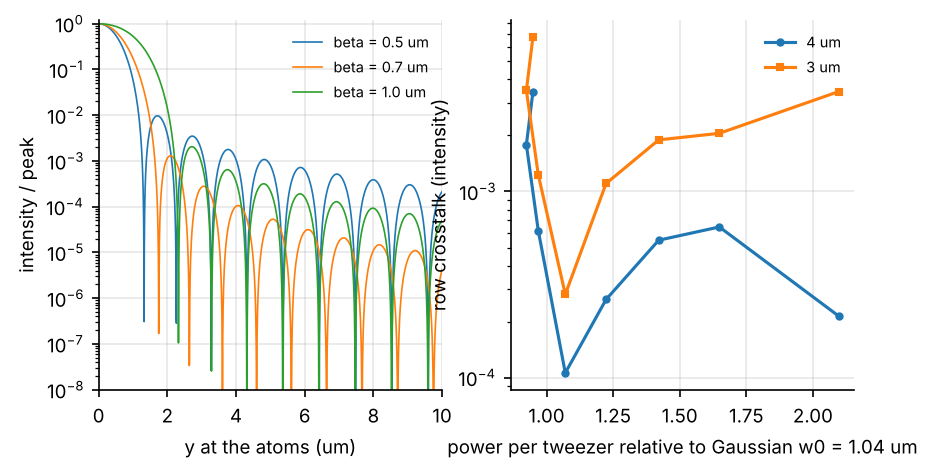
\includegraphics[width=0.85\linewidth]{m13_fill.png}
\caption{Pupil fill and row crosstalk for an ideal FAC (NA~0.9, focal length set by $\beta$, $D=125$),
scalar wave model, 1D in $y$, $s_x=0$ (valid near the row centre, see Sec.~\ref{sec:combine}). Left: $y$
intensity profile at the atoms, normalised to its peak, for $\beta=0.5$, 0.7 and 1.0~\textmu m; the facet far
field is clipped at the collimator aperture and filtered by the NA~0.5 pupil. Right: crosstalk at the
neighbouring row (3 and 4~\textmu m row pitch) against the power per tweezer relative to a Gaussian cross axis
of $w_0=1.04$~\textmu m, for $\beta$ from 0.5 to 1.0~\textmu m. The minimum at power factor 1.07 is
$\beta=0.7$~\textmu m.}
\label{fig:rows-fill}
\end{figure}

At $\beta = 0.7$~\textmu m the $y$ spot is 1.31~\textmu m FWHM, against 1.22~\textmu m for the Gaussian
assumed so far. Together with the 2.7\% cross-axis loss and a 3\% loss to the circular pupil, the power per tweezer rises
by a factor 1.10, the same at the field centre and edge. This raised the power per 1.2~mK tweezer from the
43~mW of the engine design (Gaussian cross axis) to 47~mW. The emitter facet loss found with the real
collimator raises it further, to 57~mW (Sec.~\ref{sec:rows-collimator}).

\subsection{The adopted collimator and the facet loss}\label{sec:rows-collimator}

A collimator must bend rays from $\sin\theta=0.9$ (64$^\circ$ in air) to the axis within a lens no taller
than the 0.5~mm chip pitch, with focal length 175~\textmu m. Single refracting surfaces fail for three
reasons: (i) a plano-hyperbolic lens with its curved side to the facet collimates exactly, but only up to
$\sin\theta=\sqrt{1-1/n^2}$, i.e.\ 0.72 for fused silica and 0.83 for $n=1.8$; (ii) a plano-asphere with its
flat side to the facet reaches NA~0.9, but rays meet its surfaces at up to 43$^\circ$ (fused silica, close to
total internal reflection) or 64$^\circ$ ($n=1.8$, 51\% bare transmission at the flat face); (iii) a single
elliptical surface on a block glued to the facet collimates exactly up to NA $\sqrt{n^2-1}=1.05$, but violates
the sine condition, so that the ray at $s=0.9$ exits at 68\% of the height an aplanatic lens would give.
Here, $s=\sin\theta$ at the facet and $n$ is the lens index.

The Weierstrass construction resolves this. A circular surface of radius $R$ on a glass block, with the facet
at $R/n$ from its centre, is aplanatic: every ray appears to come without aberration from a virtual point, and
the NA drops by $n^2$ (from 0.9 to 0.43 for fused silica). A second lens of focal length
$f_\mathrm{FAC}\,n^2 = 368$~\textmu m then collimates NA~0.43. We design it as a two-asphere aplanat in 2D
(Wassermann-Wolf construction: exact collimation and exact sine condition). A scan of $R$, the air gap, the
aplanat thickness and its index (96 combinations, 29 reaching NA~0.9) selected $R=80$~\textmu m, a
10~\textmu m gap, a 250~\textmu m thick aplanat and $n=1.8$. This combination gives the lowest largest
incidence angle (25.4, 18.2 and 19.2$^\circ$ on the three surfaces). Ray traced, it collimates to NA~0.9 with a
sine-condition error below $4\times10^{-5}$ over the aperture and no residual wavefront error. The lens is
395~\textmu m long (facet to last vertex) with a clear height of $\pm158$~\textmu m. Figure~\ref{fig:rows-designs}
and Table~\ref{tab:rows-designs} compare it with the single-surface alternatives.

\begin{figure}[htbp]\centering
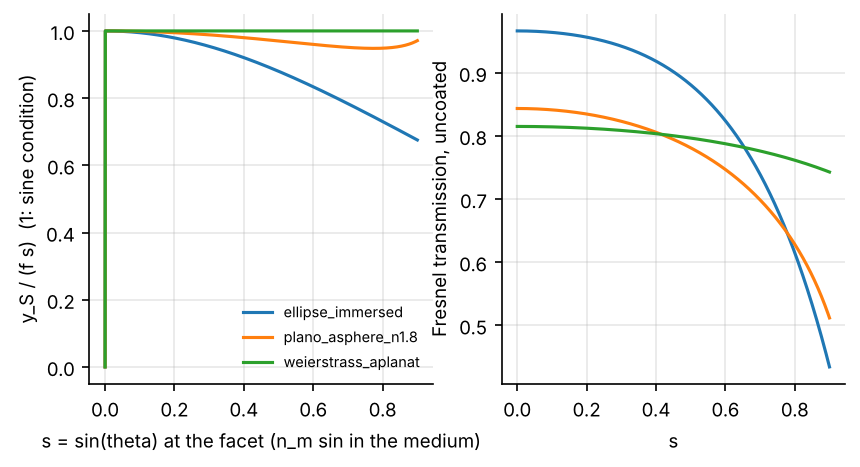
\includegraphics[width=0.85\linewidth]{m14_designs.png}
\caption{Ray-traced collimator designs (2D, cylindrical), focal length 175~\textmu m, NA~0.9. Left: sine
condition, exit height $y_S$ divided by $f\,s$, against the direction sine $s$ at the facet (in the medium for
the glued designs); 1 means aplanatic. Right: Fresnel transmission of the uncoated lens surfaces against $s$.
Designs: ellipse on a glued (immersed) block, plano-asphere of index 1.8 in air, and the adopted Weierstrass
block (fused silica, $R=80$~\textmu m) with a 10~\textmu m gap and a 250~\textmu m aplanat of index 1.8.
The wave model uses AR-coated surfaces.}
\label{fig:rows-designs}
\end{figure}

\paragraph{Facet loss.} The $x$ model of the chip treated the emitter facet as lossless, and the cross-axis
model above normalised to the power radiated into air. A Kirchhoff estimate puts the loss into air at 27\%, from
8\% Fresnel reflection plus the 20\% of the angular spectrum of the 0.39~\textmu m vertical mode that lies
beyond the light cone. We checked this with a 2D FDTD (MEEP, resolution 40/\textmu m) of the vertical
cross-section, with the SiN core index set to 1.965 so that the slab mode index equals that of the 3D mode
(1.7995). Into air, the facet reflects 12.8\% back into the chip and transmits 79.1\%, of which 77.2\% of the
guided power lies within the collimator aperture ($|s|<0.9$; Kirchhoff 72.3\%). Into fused silica, as for the
glued Weierstrass block, it reflects 2.3\% and transmits 95.9\%, with 85.2\% within the aperture (Kirchhoff
82.9\%). The remainder (8\% in air, 2\% in glass) leaves through the cladding near the facet. The emitter facet
thus loses about a quarter of the light into air, a loss absent from all earlier power figures. Gluing the
collimator to the facet recovers about 10\% and cuts the back-reflection sixfold. This is a 2D result with
the lateral confinement folded into the core index; a 3D FDTD of the facet has not been done.

\begin{table}[htbp]\centering\small
\caption{Collimator designs in the wave model (FDTD-scaled facet spectrum, AR-coated lens surfaces, NA~0.5
pupil, $s_x=0$). Peak is per unit guided power relative to the ideal lens in air at $\beta=0.7$~\textmu m.
Power is the laser power per 1.2~mK tweezer, field mean. Simulated.}
\label{tab:rows-designs}
\begin{tabularx}{\linewidth}{Xcccccc}
\toprule
design & sine condition at & largest & $\beta$ & peak & crosstalk at & power per \\
 & $s=0.3$ / 0.6 / 0.9 & incidence & (\textmu m) & & 3 / 4~\textmu m & tweezer \\
\midrule
ideal lens, air & 1 / 1 / 1 & & 0.7 & 1.00 & $2.8\times10^{-4}$ / $1.1\times10^{-4}$ & 61~mW \\
\textbf{Weierstrass + aplanat, glued} & 1.000 / 1.000 / 1.000 & 25$^\circ$ & 0.7 & \textbf{1.10} & $4.0\times10^{-4}$ / $8.0\times10^{-5}$ & \textbf{57~mW} \\
ellipse, printed & 0.954 / 0.834 / 0.675 & 43$^\circ$ & 0.9 & 1.03 & $6.6\times10^{-4}$ / $1.8\times10^{-4}$ & 61~mW \\
ellipse, printed & as above & 43$^\circ$ & 0.7 & 1.22 & $2.1\times10^{-3}$ / $1.0\times10^{-3}$ & \\
plano-asphere $n=1.8$, air & 0.988 / 0.960 / 0.971 & 64$^\circ$ & 0.7 & 1.03 & $4.0\times10^{-4}$ / $1.7\times10^{-4}$ & 59~mW \\
\bottomrule
\end{tabularx}
\end{table}

The aplanatic design reproduces the ideal lens in glass exactly (peak 1.10; a 2D check gives 1.107), with a
$y$ FWHM of 1.35~\textmu m. The ellipse narrows the $y$ spot (1.13~\textmu m at $\beta=0.7$~\textmu m) because
its mapping compresses the outer far field, but the same distortion raises the crosstalk to
$1.0\times10^{-3}$ at 4~\textmu m. Opening the fill to $\beta=0.9$~\textmu m restores $1.8\times10^{-4}$ at a
cost of 15\% in peak. Without AR coatings all designs lose 10 to 30\% ($n=1.8$ surfaces reflect 8\% each at
normal incidence), so coatings are needed in every case. With the adopted collimator the power per 1.2~mK
tweezer is 57~mW, against 47~mW with the facet loss omitted and 61~mW for an ideal lens in air.

\paragraph{The first $x$ lens.} The first lens of the $x$ relay ($f=3.12$~mm, NA~0.355 through the slit)
sees the whole emitter row, $\pm144$~\textmu m, and works off axis. We traced two fused-silica designs from
seven emitter heights and applied each off-axis wavefront to the emitters' angular spectra in the D1 model.
An aplanat has 0.15 waves rms at the 144~\textmu m field (tilt removed). Uncalibrated, its edge tweezer reaches
0.960 of the peak and is shifted by 164~nm; after least-squares recalibration it reaches 1.001 per unit power
with a shift of at most 1.5~nm. A plano-asphere without the sine condition (0.60 waves rms) recovers 0.964 after
recalibration. The static aberration of the $x$ relay is a fixed linear transformation of the chip's response,
and the least-squares synthesis, which already works on the measured response matrix, removes it. The $x$
relay therefore needs ordinary lens quality. The same argument does not apply to the collimator, because the
$y$ axis has no actuators.

\subsection{Crosstalk between rows}\label{sec:rows-crosstalk}

For the 2D test, chip $m$ forms a full row of 41 tweezers at 3~\textmu m spacing over $\pm60$~\textmu m, with
alternating phases 0 and $\pi/2$. The neighbouring chip forms 11 tweezers offset by 1.5~\textmu m in $x$. We
evaluate the pair at row separations of 3 to 16~\textmu m, with the ideal FAC and $s_x=0$. ``Coherent'' means
both chips use one laser frequency, with the worst of eight relative phases; ``incoherent'' means their
relative phase is averaged out. Table~\ref{tab:rows-crosstalk} and Fig.~\ref{fig:rows-crosstalk} give the
results.

\begin{table}[htbp]\centering\small
\caption{Crosstalk between neighbouring rows in 2D (ideal FAC, $\beta=0.7$~\textmu m, $s_x=0$). Full-row
crosstalk is the intensity of a full row of 41 tweezers at the neighbouring row relative to the peak (maximum
over $x$). Static: change of depth / position of a neighbouring tweezer when the full row is switched on.
Moving: change when one tweezer of row $m$ moves by 0.25~\textmu m. Simulated.}
\label{tab:rows-crosstalk}
\begin{tabular}{cccccc}
\toprule
row & full-row & \multicolumn{2}{c}{incoherent rows} & \multicolumn{2}{c}{coherent rows} \\
separation & crosstalk & static & moving & static & moving \\
\midrule
3~\textmu m & $4.3\times10^{-4}$ & $2.0\times10^{-4}$ / 0.13~nm & $6.2\times10^{-5}$ / 0.04~nm & 2.9\% / 18~nm & $6.5\times10^{-3}$ / 5.6~nm \\
4~\textmu m & $1.8\times10^{-4}$ & $1.7\times10^{-4}$ / 0.002~nm & $2.4\times10^{-5}$ / 0.04~nm & 2.6\% / 11~nm & $2.8\times10^{-3}$ / 4.5~nm \\
6~\textmu m & $6.3\times10^{-5}$ & $4\times10^{-6}$ / 0.02~nm & $3\times10^{-6}$ / 0.01~nm & 0.41\% / 8.9~nm & $1.7\times10^{-3}$ / 2.1~nm \\
8~\textmu m & $4.3\times10^{-5}$ & $<10^{-6}$ & $<10^{-6}$ & 0.08\% / 1.8~nm & $1.1\times10^{-3}$ / 1.7~nm \\
12~\textmu m & $1.5\times10^{-5}$ & $<10^{-6}$ & $<10^{-6}$ & 0.01\% / 5.9~nm & $8\times10^{-4}$ / 0.8~nm \\
16~\textmu m & $1.3\times10^{-5}$ & $2\times10^{-6}$ & $<10^{-6}$ & 0.27\% / 1.6~nm & $4\times10^{-4}$ / 0.6~nm \\
\bottomrule
\end{tabular}
\end{table}

\begin{figure}[htbp]\centering
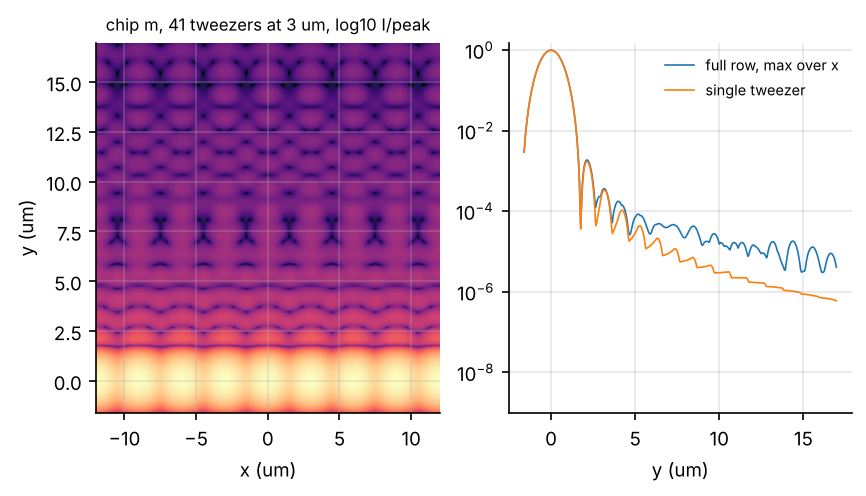
\includegraphics[width=0.85\linewidth]{m13_crosstalk.png}
\caption{Light from one chip at the neighbouring rows, 2D scalar model with D1's beam-propagation response in
$x$ and the facet mode through an ideal NA~0.9 FAC in $y$ ($\beta=0.7$~\textmu m, $s_x=0$, valid near the row
centre). Left: $\log_{10}$ of the intensity relative to the peak for a full row of 41 tweezers at
3~\textmu m spacing, alternating phases 0 and $\pi/2$, shown over $|x|\le12$~\textmu m. Right: maximum over
$x$ of the full row's intensity against $y$, compared with a single tweezer. The full row has a tail plateau
of about $10^{-5}$ out to 16~\textmu m.}
\label{fig:rows-crosstalk}
\end{figure}

With incoherent rows, a moving tweezer changes the next row by at most $6\times10^{-5}$ in depth and
0.04~nm in position, even at 3~\textmu m row pitch. This is two orders of magnitude below the in-row figures of
D1 (0.11\%, 3.5~nm). With coherent rows, the crosstalk field $\epsilon$ (in intensity) interferes with the
neighbour's own field, so the depth changes by about $2\sqrt{\epsilon}\cos\phi$. Here, $\phi$ is the relative
optical phase of the two chip feeds. This interference persists at all simulated distances because of the
tail plateau of a full row. Its strength follows $\phi$, which drifts with temperature and acoustics in the
separate fibre paths, so the 2.6\% and 11~nm at 4~\textmu m become slow, uncontrolled noise. Alternating two
frequencies between neighbouring chips is therefore not enough. In the original plan of the study every chip
ran at its own frequency, with pairwise differences of at least 1~MHz, far above twice the 84~kHz trap
frequency: one acousto-optic shifter per chip feed at $80 + 1.13\,m$~MHz ($m=0$ to 15), each handling 2.6 to
3.4~W (handling at this power: [VALUE?]). The beat notes then modulate the depth at MHz rates with amplitude
about $2\sqrt{\epsilon}$, which the atoms average. The next subsection replaces these 16 shifters. The tweezers
within one row stay coherent in either scheme, as the least-squares synthesis of the engine requires.

\subsection{Decorrelating the rows without frequency shifters}\label{sec:rows-decorrelate}

A frequency offset $\delta f$ makes $\phi$ advance at $2\pi\,\delta f$, and the atom sees only the time
average when $\delta f$ is far above the trap frequencies. Any process that randomises $\phi$ on time scales
much shorter than the trap period does the same. We use a common random phase seen with different delays. If
the seed carries a phase $\varphi(t)$ and chip $m$ receives it after a delay $\tau_m$, the relative phase of
chips $m$ and $n$ is $\varphi(t-\tau_m)-\varphi(t-\tau_n)$. Its mean contribution to the interference is the
field coherence $|\langle \exp\{i[\varphi(t)-\varphi(t-\tau)]\}\rangle|$ at $\tau=\tau_m-\tau_n$.

Our choice of modulation is a compromise between residual coherence and tolerance to real hardware. A binary
$0/\pi$ m-sequence ($N=1023$) leaves $9.8\times10^{-4}=1/N$ at integer delays. However, every transition passes
through $+\pi/2$, so a modulator with a 10--90\% rise of 0.3 bit leaves a carrier of 0.12 and a residual
coherence of $4.1\times10^{-2}$, and a depth error of 5\% (10\%) gives $5.2\times10^{-3}$
($2.4\times10^{-2}$). A Zadoff-Chu polyphase code ($N=1021$) has perfect autocorrelation but needs exact delays
($6.2\times10^{-2}$ at non-integer ones). Gaussian phase noise of $\sigma=3$~rad rms needs neither: the carrier
is $\exp(-\sigma^2/2)$, and any delay longer than about three correlation times decorrelates. Its residual
coherence is $1.2\times10^{-4}$ in the ensemble ($\exp(-9)$), and 4.2 to $7.2\times10^{-3}$ in our
32,768-bit simulated records, which is their statistical floor. What the atom sees is set by the low-frequency
density of the interference term, $0.40/B$, where $B$ is the correlation rate of the noise. For the coherent
term $2\sqrt{\epsilon}=2.1\times10^{-2}$ this gives a relative intensity noise density
$S_I(2\nu_\mathrm{trap})=8.8\times10^{-14}$/Hz at $B=2$~GHz. The parametric heating rate
$\Gamma=\pi^2\nu^2 S_I(2\nu)$ \cite{OHARA} is then $6\times10^{-3}$~s$^{-1}$ at $\nu=84$~kHz, an energy
e-folding time above 2 minutes; at $B=0.5$~GHz it is $2.4\times10^{-2}$~s$^{-1}$.

The adopted scheme is therefore one fibre-coupled LiNbO$_3$ phase modulator on the low-power seed, ahead of the
1:16 split, driven by a Gaussian noise source amplified to about $1\,V_\pi$ rms (3~rad) over 1 to 2~GHz. The
16 chip feeds receive 0, 0.3, 0.6, \ldots, 4.5~m of extra fibre (steps of at least three correlation lengths at
2~GHz). Within one chip and its relay, path differences are at most about 1~mm (about 5~ps). With a 0.5~ns
correlation time and $\sigma=3$~rad the coherence loss is $\sigma^2(\tau/\tau_c)^2/2\approx5\times10^{-4}$,
so the synthesis sees an essentially coherent source. The optical spectrum becomes Gaussian with rms width
$0.67B$ (1.35~GHz, 5~pm, at $B=2$~GHz). Through the diffractive objective's axial chromatic shift
(16~\textmu m/nm, derived for $f_\mathrm{obj}\propto1/\lambda$) this smears the focus by 0.08~\textmu m rms
(peak 0.9998) and the lateral position at 60~\textmu m by 0.29~nm rms. The spectrum is symmetric, so the mean
light shift at the double-magic wavelength is unchanged to first order; the second-order term needs the
curvature of the differential polarisability, which we do not have [VALUE?]. A seed broadened to about 1~GHz
also raises the stimulated-Brillouin threshold of the high-power amplifier and the delivery fibres, which
carry about 3~W each ([REF?]; recalled: SBS suppression by phase modulation is standard in high-power
single-frequency fibre amplifiers). If the chosen amplifier already broadens its seed for this reason, the only
addition is the fibre delays. Compared with 16 acousto-optic shifters, the scheme removes 16 RF drivers and the
shifter insertion loss (about 15\% each [VALUE?]).

\begin{table}[htbp]\centering\small
\caption{Options for row independence: perturbation of a tweezer by all other rows within $\pm16$~\textmu m
(both sides; rms over drifting relative phases, pairs in quadrature; 4~\textmu m rows, full rows of 41
tweezers; $s_x=0$). Criteria used for tweezers within a chip: others' depth change $<3\times10^{-3}$ and
position change $<5$~nm when a tweezer moves; position noise budget of the proposal 10~nm rms. Simulated
(vector focusing for the polarisation options) and derived.}
\label{tab:rows-options}
\begin{tabularx}{\linewidth}{lXccc}
\toprule
option & added hardware & power & static: depth / position & moving 0.25~\textmu m: depth / position \\
\midrule
all chips coherent & none & 1 & 2.3\% / 9.2~nm & $2.3\times10^{-3}$ / 5.1~nm \\
per-chip frequency offsets & 16 shifters at 2.6 to 3.4~W & 1 (+ shifter loss) & $1.8\times10^{-4}$ / 0.09~nm & $2\times10^{-5}$ / 0.05~nm \\
\textbf{phase noise + delays} & \textbf{1 modulator on the seed, noise source, $\le5$~m fibre} & \textbf{1} & $\mathbf{1.6\times10^{-4}}$ / \textbf{0.07~nm} & $\mathbf{2\times10^{-5}}$ / \textbf{0.04~nm} \\
alternating $x$/$y$ polarisation & half-wave-plate strips (passive) & 1 & $4.2\times10^{-3}$ / 2.5~nm & $1.1\times10^{-3}$ / 1.6~nm \\
$y$ apodiser, $a=0.65$ & graded mirror (passive) & 1.84 & $5.2\times10^{-3}$ / 4.1~nm & $1.0\times10^{-3}$ / 1.8~nm \\
polarisation + apodiser $a=0.8$ & passive & 1.55 & $2.8\times10^{-3}$ / 1.8~nm & $5.7\times10^{-4}$ / 0.7~nm \\
\bottomrule
\end{tabularx}
\end{table}

As can be seen from Table~\ref{tab:rows-options}, common phase noise with fibre delays gives the same row
independence as per-chip frequency offsets, at no power penalty. Leaving all chips coherent breaks the
position budget: 9.2~nm rms of slow wander plus 5.1~nm when neighbours move.

\paragraph{Passive alternatives.} A half-wave-plate strip in front of every other chip, in the collimated region
after the collimators, gives alternate rows orthogonal linear polarisation. Vector focal fields (Richards-Wolf,
aplanatic NA~0.5 objective, intensity summed over $E_x$, $E_y$ and $E_z$) show that the interference of
orthogonal neighbours falls by a factor of 26; the residual comes from the depolarisation of high-angle rays,
mainly via $E_z$. Rows two apart (8~\textmu m) share a polarisation and then dominate. The moving-tweezer
criteria and the position budget are met, but the static depth wanders by 0.4\% rms with the fibre phases at
Hz to kHz rates. The option has three costs: (i) the meta-objective must be polarisation-insensitive
(propagation-phase meta-atoms with fourfold symmetry rather than geometric phase); (ii) where the orthogonal
fields overlap, the polarisation becomes elliptical in proportion to their relative phase, which produces a
vector light shift. With a vector-to-scalar ratio of about $0.09\,g_F m_F$ per unit ellipticity (recalled, to
be verified, from the far-detuned formula \cite{GRIMM}) and an ellipticity of up to about $2\times10^{-2}$ at
4~\textmu m, this is about $2\times10^{-3}\,g_F m_F$ of the trap depth: up to tens of kHz for stretched states
and zero to first order for clock states ($m_F=0$); (iii) only two orthogonal states exist, so rows two apart
stay coherent. A passive Gaussian apodiser at the $y$ telescope plane conjugate to the pupil lowers the 1D
crosstalk at 4~\textmu m from $8.4\times10^{-5}$ to $3.5\times10^{-6}$ ($a=0.65$ pupil radii), but it costs a
factor 1.84 in power, widens the $y$ spot from 1.35 to 1.73~\textmu m, and in 2D still leaves
$4.7\times10^{-3}$ of static depth change at 4~\textmu m. It is not competitive. We adopt the phase noise with
fibre delays. Alternating polarisation costs nothing to add and gives a second, independent factor of about 26
on the nearest rows if the modulation fails or is switched off.

\subsection{Conversion of phase noise to intensity noise}\label{sec:rows-pmam}

Phase noise alone leaves the intensity constant (the simulated control gives $-376$~dB/Hz, the numerical
floor). Intensity noise appears only where an element filters the spectrum. We simulated each element of a
laser chain separately on the modulated field ($\sigma=3$~rad, $B=2$~GHz; record 131~\textmu s at 16~GS/s; for
delayed copies, the worse of two relative phases). The criterion is a parametric heating rate
$\Gamma\le0.1$~s$^{-1}$ at $\nu=84$~kHz (energy doubling time about 7~s), i.e.\ a relative intensity noise
(RIN) density at 168~kHz of $S\le1.4\times10^{-12}$/Hz ($-118$~dB/Hz). Table~\ref{tab:rows-pmam} gives the
results.

\begin{table}[htbp]\centering\small
\caption{Phase-to-intensity conversion by individual elements of the laser chain (Gaussian phase noise
3~rad rms, $B=2$~GHz). RIN rms is over all frequencies (mostly at GHz); the density is at 168~kHz $=2\nu_\mathrm{trap}$.
Element parameters are chosen ranges, not component data; PM-fibre group delay 1.2~ps/m and dispersion
20~ps$^2$/km are recalled, to be verified. Simulated.}
\label{tab:rows-pmam}
\begin{tabularx}{\linewidth}{Xccc}
\toprule
element & RIN rms & RIN at 168~kHz & $\Gamma$ (s$^{-1}$) \\
\midrule
amplifier gain tilt, 0.05 / 0.5 / 5~dB/nm & $6\times10^{-5}$ / $6\times10^{-4}$ / $6\times10^{-3}$ & $-237$ / $-216$ / $-182$~dB/Hz & $<10^{-6}$ \\
band-pass 1~nm FWHM, offset 250~pm (ASE filter) & $7\times10^{-3}$ & $-173$~dB/Hz & $<10^{-6}$ \\
band-pass 100~pm, centred / offset 25~pm & $1.0\times10^{-2}$ / $7.0\times10^{-2}$ & $-130$ / $-133$~dB/Hz & $7\times10^{-3}$ / $3\times10^{-3}$ \\
band-pass 30~pm, centred / offset 7.5~pm & $9.6\times10^{-2}$ / 0.21 & $\mathbf{-110}$ / $\mathbf{-113}$~dB/Hz & \textbf{0.70} / \textbf{0.37} \\
multipath $R_1=R_2=10^{-2}$, delay $\ge0.3$~ns & $1.4\times10^{-2}$ & $-130$~dB/Hz & $7\times10^{-3}$ \\
multipath $R_1=R_2=10^{-2}$, delay 0.1 / 0.01~ns & $7\times10^{-3}$ / $10^{-4}$ & $-133$ / $-171$~dB/Hz & $3\times10^{-3}$ / $10^{-6}$ \\
multipath $R_1=R_2=10^{-3}$ or $10^{-4}$, any delay & $\le1.4\times10^{-3}$ & $\le-149$~dB/Hz & $\le8\times10^{-5}$ \\
PM fibre, extinction $-20$~dB, 5 / 20~m, then TE guide & $3\times10^{-4}$ / $5\times10^{-3}$ & $-161$ / $-137$~dB/Hz & $6\times10^{-6}$ / $1.4\times10^{-3}$ \\
dispersion, 5~m to 1~km & $\le8\times10^{-4}$ & $<-280$~dB/Hz & 0 \\
representative chain & $6.9\times10^{-3}$ & $-134.5$~dB/Hz & $2.5\times10^{-3}$ \\
\bottomrule
\end{tabularx}
\end{table}

The structure follows from the physics. Gain tilt and dispersion respond to the instantaneous frequency, the
time derivative of the phase, whose spectrum vanishes towards low frequency, so their intensity noise lies at
GHz. A delayed copy of amplitude $r$ produces an intensity term $2r\cos[\varphi(t)-\varphi(t-\tau)]$. Once
$\tau$ exceeds the correlation time (about 0.3~ns), this term is a random, telegraph-like signal of variance
$2r^2$ spread over about $B$, so $S\approx4r^2\times0.40/B$ (Fig.~\ref{fig:rows-pmam}). For $\tau$ far below
the correlation time the term is quadratic in the phase increment and much smaller. A band-pass filter
narrower than the spectrum acts as the same effect distributed over its impulse response, about
$1/(\pi\,\mathrm{FWHM}) = 40$~ps for 30~pm. The dependence on $B$ cuts both ways: at $r=10^{-2}$ and
$\tau=1$~ns, $S$ is $-125$, $-130$ and $-138$~dB/Hz for $B=0.5$, 2 and 8~GHz, whereas at $\tau=0.1$~ns
$B=0.5$~GHz is the quietest ($-170$~dB/Hz) because the copy still lies inside the correlation time. We keep
$B=2$~GHz as a middle value.

\begin{figure}[htbp]\centering
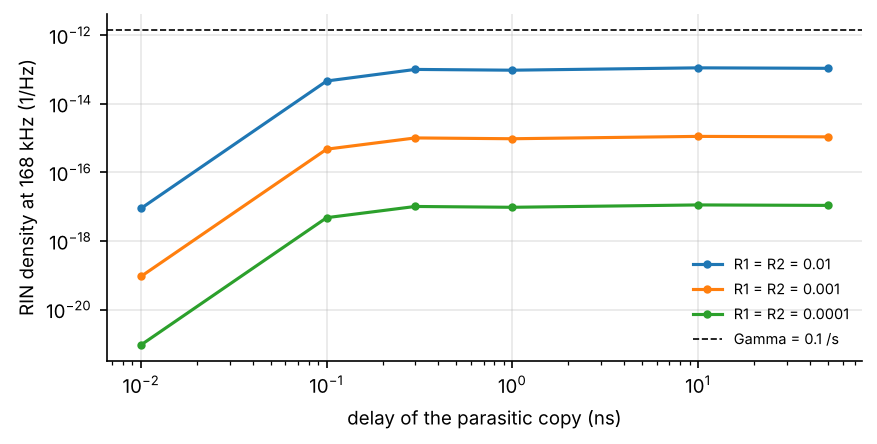
\includegraphics[width=0.8\linewidth]{m16_pm_am.png}
\caption{RIN density at 168~kHz ($2\nu_\mathrm{trap}$) produced by one parasitic delayed copy from two
reflections $R_1=R_2$, against the delay of the copy, for Gaussian phase noise of 3~rad rms at $B=2$~GHz
(simulated record 131~\textmu s at 16~GS/s, worse of two relative phases). Dashed line: the criterion
$\Gamma=0.1$~s$^{-1}$ at $\nu=84$~kHz ($1.4\times10^{-12}$/Hz). Beyond about 0.3~ns the density saturates at
$\approx4r^2\times0.40/B$ with $r^2=R_1R_2$.}
\label{fig:rows-pmam}
\end{figure}

Two design rules follow: (i) no filter narrower than about 100~pm (20 times the 1.35~GHz rms modulation width)
in the light path; (ii) the product of any two reflections in the chain below $R_1R_2=1.7\times10^{-3}$
(amplitude $r\le0.042$), i.e.\ no pair of uncoated glass surfaces in series. A representative chain (amplifier
tilt 0.5~dB/nm; ASE filter of 1~nm FWHM offset by 250~pm; 5~m of PM fibre with $-20$~dB polarisation
crosstalk; two $-30$~dB connector reflections 5~m apart; an on-chip etalon between a $-30$~dB input facet and
the 2.3\% glued emitter facet, 190~ps round trip; 5~m of dispersion) gives $-134.5$~dB/Hz and
$\Gamma=2.5\times10^{-3}$~s$^{-1}$ (energy e-folding about 7~min), 16~dB inside the criterion. The on-chip
etalon and the connector pair dominate. Without modulation, the same reflections produce no noise at 168~kHz.
Instead they give a slow intensity offset $2r\cos\Phi$ that follows the drift of the path phase $\Phi$: 2\% for
$r=10^{-2}$, at Hz to kHz rates. The modulation converts this offset into broadband noise of the same rms, of
which only $10^{-13}$ to $10^{-12}$/Hz lands near the trap frequencies. The phase noise therefore also helps
against parasitic etalons, provided rule (ii) holds. The elements are linear and treated separately; amplifier
gain dynamics, self-phase modulation and stimulated Brillouin scattering are not modelled. The prediction to
test is a RIN floor below $-130$~dB/Hz at 10~kHz to 1~MHz after the full amplified chain, with a 1~nm ASE
filter and AR-coated components, with the modulation on and off.

\subsection{Alignment, assembly and drift}\label{sec:rows-align}

Table~\ref{tab:rows-tol} gives per-chip errors for a single tweezer at $x=0$ with the ideal collimator (the
field edge, $x=60$~\textmu m, gives the same values within 0.1\% at $s_x=0$). None of these errors moves the
row in $y$ by more than 0.01~nm.

\begin{table}[htbp]\centering\small
\caption{Alignment tolerances of one chip and its FAC (ideal collimator, 2D, $s_x=0$). Peak is at the nominal
atom plane relative to no error; crosstalk is the worst value at the 4~\textmu m neighbour (no error:
$1.1\times10^{-4}$, $y$ FWHM 1.33~\textmu m). Simulated.}
\label{tab:rows-tol}
\begin{tabular}{lccc}
\toprule
error & value & peak & crosstalk at 4~\textmu m \\
\midrule
FAC decentre in $y$ & 0.05 / 0.1 / 0.2 / 0.3~\textmu m & 0.992 / 0.969 / 0.881 / 0.750 & $2\times10^{-4}$ / $4\times10^{-4}$ / $1.2\times10^{-3}$ / $2.8\times10^{-3}$ \\
FAC focus along $z$ & 0.25 / 0.5 / 1 / 2~\textmu m & 0.993 / 0.973 / 0.893 / 0.641 & $3\times10^{-4}$ / $9\times10^{-4}$ / $2.8\times10^{-3}$ / $4.3\times10^{-3}$ \\
FAC roll about $z$ & 0.5 / 1 / 2~mrad & 0.998 / 0.992 / 0.968 & $10^{-4}$ / $10^{-4}$ / $2\times10^{-4}$ \\
smile (bow, peak to valley) & 0.1 / 0.2 / 0.4~\textmu m & 0.998 / 0.992 / 0.967 & $10^{-4}$ / $2\times10^{-4}$ / $4\times10^{-4}$ \\
FAC wavefront, spherical-like & 0.05 / 0.1 waves rms & 0.942 / 0.783 & $3\times10^{-4}$ / $1.2\times10^{-3}$ \\
FAC wavefront, coma-like & 0.05 / 0.1 waves rms & 0.937 / 0.767 & $5\times10^{-4}$ / $2.0\times10^{-3}$ \\
chip piston along $z$ & 10 / 100 / 300~\textmu m & $\ge0.999$ / $\ge0.992$ / $\ge0.908$ & \\
\bottomrule
\end{tabular}
\end{table}

The collimator decentre is the tightest tolerance: $\pm0.1$~\textmu m for 3\% loss. A decentre $\delta$ shifts
the facet image in the pupil by $\delta/\beta$ of the pupil radius, so the tolerance scales with the vertical
facet mode. It costs power and crosstalk but does not move the row. The ray-traced designs confirm that it is a
property of the facet, not of the lens: $\pm0.1$~\textmu m for every design (peak 0.973 at 0.1~\textmu m and
0.896 at 0.2~\textmu m for the adopted collimator). Focus is looser for the glued designs because the facet
radiates into glass (the defocus phase scales as $n_m\cos\theta$, with $n_m$ the medium index): about
$\pm1$~\textmu m for 3\% for the adopted collimator, against $\pm0.5$~\textmu m for the ideal lens in air. The
wavefront requirement (about 0.03 waves rms for $\le3\%$ at NA~0.9) follows from the same imaging: the collimator
is the aperture of the facet-to-pupil image, and light it scatters out of that image misses the pupil. For the
adopted collimator this translates into a surface form error of at most 20~nm rms for $\le2\%$ loss (mean peak
0.984 at 20~nm and 0.916 at 50~nm rms, correlation length 20~\textmu m). A chip piston of 10, 100 and 300~\textmu m
moves the $x$ position statically by at most 1.5, 0.9 and 6.8~nm, so facets must stay flush to within about
100~\textmu m. Stair-step stacking for wire bonds is therefore excluded, and fibre and electrical access must
come from the chip sides or back; this access is not addressed here.

The row positions at the atoms follow from the conjugations (derived). A height error of chip plus collimator,
or a placement error of the collimator, moves its row by $1/D = 8$~nm per \textmu m. A chip tilt about $x$ of
1~mrad moves the row by $f_\mathrm{FAC}\times1~\mathrm{mrad}/D=1.4$~nm. A chip piston $\mathrm{d}z$ defocuses
its row in $y$ by $\mathrm{d}z/D^2$ (6~nm per 100~\textmu m). A stack built to $\pm2$~\textmu m therefore places
rows to $\pm16$~nm; a static offset of this size must be matched by the static 1075~nm array, or measured and
absorbed into its design.

Drift sets the mounting. For a collimator glued to its own facet, vertical registration is fixed at the facet,
and differential expansion acts only over the lens's own height ($\pm80$~\textmu m at the glued block). With
$\Delta\alpha\approx2\times10^{-6}$/K (Si $2.6\times10^{-6}$/K against fused silica $0.55\times10^{-6}$/K,
recalled, to be verified) this is about 0.2~nm/K. A monolithic collimator array for the whole stack, referenced
at its base, would see the full 8~mm stack height: 16~nm/K at the top chip, so 0.1~\textmu m after 6~K. Hence
one collimator per chip, or a stack held to $\pm1$~K. Thermal expansion of the Si stack itself moves the outer
rows by about 0.2~nm/K at the atoms. The glue line of the immersed design lies along $z$, so cure shrinkage
changes mainly the focus ($\pm1$~\textmu m tolerance) and only weakly the decentre; the vertical position must
nevertheless be held to $\pm0.1$~\textmu m during cure, and the shrinkage and creep of UV adhesives at this level
need a source [REF?]. The alignment signal is strong: a decentre moves the facet image across the pupil by
$\delta\times12{,}400$, so 0.1~\textmu m becomes 1.2~mm on the 17~mm pupil, and a camera with 10~\textmu m pixels
imaging the pupil (or its conjugate in the $y$ telescope) resolves 1~nm of decentre in principle. Active
alignment against this signal, before and during cure, is the process we recommend. A collimator printed by
two-photon lithography directly on the facet would be registered lithographically; its placement accuracy
needs a source [REF?], as do the achievable wavefront error of NA~0.9 micro-collimators [REF?] and the
long-term stability of actively aligned, bonded collimators [REF?].

\subsection{Power and laser plan for 16 chips}\label{sec:rows-power}

Table~\ref{tab:rows-power} gives the power plan with the adopted collimator (57~mW per 1.2~mK tweezer, field
mean, FDTD-scaled facet, AR-coated lenses), for 192-port chips (Sec.~\ref{sec:moretweezers}) with 45 tweezers
per row at 4~\textmu m spacing or 60 at 3~\textmu m.

\begin{table}[htbp]\centering\small
\caption{Laser power for 16 chips with the adopted collimator, and input fibres per chip at a facet intensity
cap of 20~MW/cm$^2$ (a design choice; no damage threshold was found). Derived.}
\label{tab:rows-power}
\begin{tabular}{cccccc}
\toprule
tweezers per row & depth & power per chip & 16 chips & \multicolumn{2}{c}{fibres per chip} \\
 & & & & lensed tip & HI1060-matched tip \\
\midrule
45 (4~\textmu m) & 1.2~mK & 2.6~W & 41~W & 5 & 1 (8~MW/cm$^2$) \\
60 (3~\textmu m) & 1.2~mK & 3.4~W & 55~W & 6 & 1 (11~MW/cm$^2$) \\
45 & 0.5~mK & 1.1~W & 17~W & 2 & 1 \\
60 & 0.5~mK & 1.4~W & 23~W & 3 & 1 \\
\bottomrule
\end{tabular}
\end{table}

Our choice of one input fibre per chip is a compromise between two considerations. First, the lensed-fibre
inverse taper of the input coupler study has a 3.1~\textmu m$^2$ mode at the chip facet, so the 20~MW/cm$^2$ cap
allows only 0.62~W per fibre and 5 to 6 fibres per chip. Several inputs would split the 128 ports into
sub-trees whose relative optical phases drift with their fibres, and a tweezer window straddling a sub-tree
boundary would then fluctuate. However, the HI1060-matched taper (tip 0.1~\textmu m, $-0.48$~dB, 0.11~dB worse
than the lensed tip) has a 30.6~\textmu m$^2$ mode and carries 6.1~W at the same cap. One fibre per chip is
therefore possible and preferred, at the cost of a 0.1~\textmu m tip width that sits at the assumed minimum
feature size. With 16 rows the stack offers 720 (4~\textmu m spacing) to 960 (3~\textmu m) independent
tweezers. The laser must deliver 41 to 55~W of single-frequency 1064.4~nm light at 1.2~mK, or 17 to 23~W at
0.5~mK; the availability of 40 to 55~W is a placeholder [VALUE?]. Lowering the
transport depth is the cheapest lever, because power scales linearly with depth and the lower trap frequency
also relaxes the required update rate (Secs.~\ref{sec:moretweezers} and~\ref{sec:transport}).

The limits of this section are as follows. The model is scalar, with ideal (sine-condition) thin cylindrical
lenses for the relay; the objective's apodisation factor and polarisation are omitted except in the vector
calculation of the polarisation option. The collimator ray trace is 2D, with ideal AR coatings in the wave
model, and the $n=1.8$ glass is a class, not a catalogue glass. The facet FDTD is 2D with an effective core
index. Tolerances are evaluated one at a time; a combined Monte Carlo of decentre, focus, form, thickness and
index has not been run. All $y$ results assume $s_x=0$ and hold near the row centre only
(Sec.~\ref{sec:combine}).
